%===================================== CHAP 7 =================================

\chapter{Project Life Cycle}

\section{Planning and Research}
The group initiated the project with a planning and research phase, lasting from January the 11th to February the 3rd. 

\subsection{Planning}
The importance of the planning phase was emphasised by the group to avoid being forced to start over because the project was insufficient according to what the customer wanted. \\

The planning phase was initiated with thoroughly choose project, focusing on the strengths and weaknesses within the group. To ensure that every member had the same ambitions and a common understating of what the group expected of each other, a group contract was also formulated. This contract has been important for the group dynamic (see apendix X). The risk analysis was also developed during the planning phase, as issues might arise unexpectedly and needs to be managed in a proper fashion (see chapter \ref{riskAnalysis}).  \\  

As the project was assigned - the group prioritised to establish contact with the customer to get a more precise idea of what was to be developed. A contract between the team and the customer was also formulated - ensuring both parties held the same expectations for the project, and of each other during the development process (see apendix X).\\

As the group achieved a better idea of what the project implied - a set of roles were created. These were delegated to the group members depending on prior experience and desire (see chapter \ref{projectOrganisation}).

\subsection{Research}
In advance of starting the development of the project a thorough research were completed.

Initially the group researched what type of methodology would suit the project, the customer and the group it self (see chapter \ref{methodology}). As the methodology was chosen the group researched what tools that facilitated an effortless use of this. The group members have a lot experience in using different tools, which opened for many opportunities for deciding what should be used (see chapter \ref{tools}).

As one of the requirements from the customer was a web portal applying the principles of universal design (see chapter \ref{universalDesign}) - and this is an aspect few of the group members has experience taking in consideration to this degree - a thorough research was completed to achieve a product applying this. The customer also provided a resource \cite{Difi} for the group the group to further investigate how this should be implemented and designed. 

The customer also provided several alternative solutions (see chapter \ref{alternativeSolutions}) for the group to investigate - primarily in how these satisfied the users' needs, or not. To serve the group the best possible understanding of the users' needs a workshop (see chapter \ref{workshop}) was arranged together with the users and providers. 


\subsubsection{Workshop With Users and Providers}
\label{workshop}
During the researching phase two of the group members, Christina and Sigve, attended a workshop. 



\section{Sprint 0}
The sprint goal for sprint 0 was "Create first design draft, planning and set up product backlog." \\

Sprint 0 did not have any user stories. Instead the sprint was used to set up the workspace, create an index template in Django, create a product backlog with the customer, decide the MVP (see chapter \ref{MVP}), create a first design draft of the application and doing as much planning as possible. The group chose to do it this way, so the development could start already in the beginning of sprint 1. \\

The design draft was drawn as a paper prototype, and the group performed a demonstration to the customer. He was satisfied with the idea, and it created a great discussion about how the group should continue working. \\

Sprint retrospective meeting summary:\\
The group are satisfied with their own efforts. Heaps of work are accomplished, and everyone are motivated to keep working next week. \\
    
The group agrees that they should be more effective in their work sessions, so they can accomplish more. To do this it is important that everyone take responsibility of keeping the group on track, and tell if people are not concentrate on the task.

\begin{figure}[h!]
\centering
    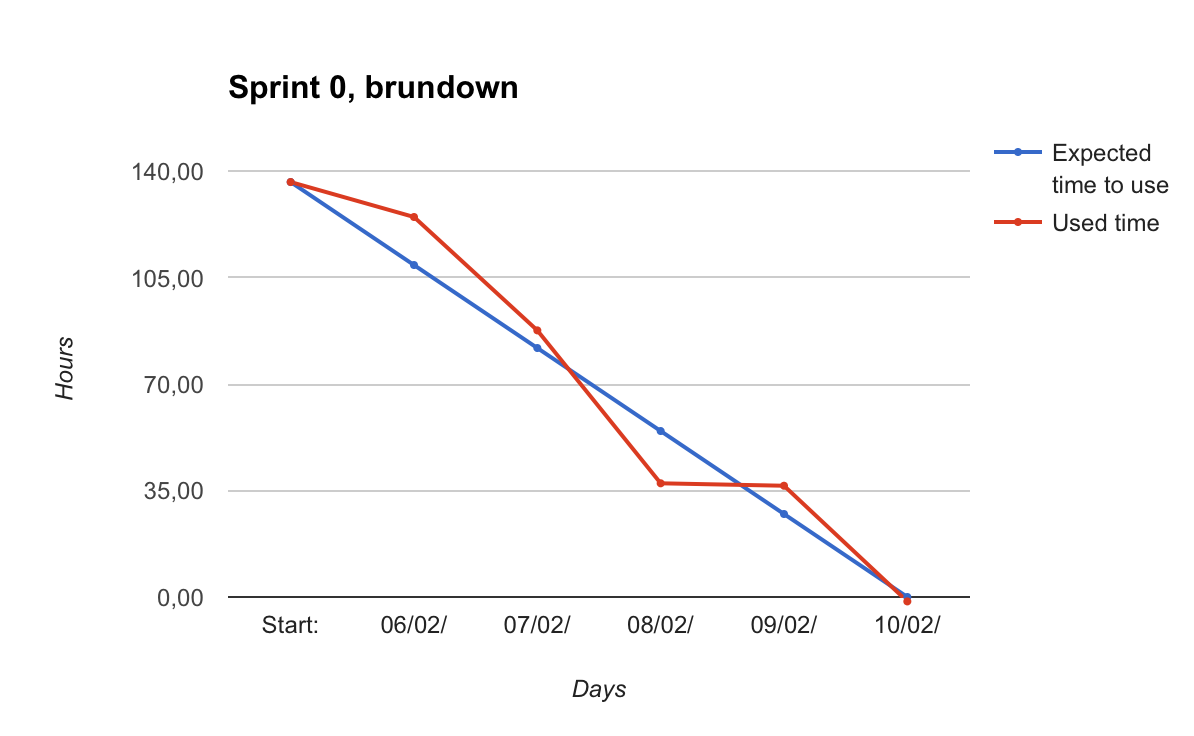
\includegraphics[width=0.8\textwidth]{fig/sprint0}
\caption{Sprint 0, burndown}
\end{figure}



\section{Sprint 1}
The sprint goal for sprint 1 was to: 
\begin{itemize}
  \item Create a mock up database.
  \item Create a flow diagram.
  \item Create issues on GitHub.
  \item Make log in, with different GUI for each role (child, parent, activity      provider, maintainer and anonymous).
  \item Log in with Facebook.
  \item Anonymous user should maybe not be able to see who is going to a activity anonymous should not be able to sign up for activity, before the user has logged in.
  \item  Site map Create skeleton for all pages in site map Investigate the possibility of changing the language (create a dynamic page where all words are listed)
  \item Update wiki (to have the flow diagram, site map and user manual)
\end{itemize}
 
There was two problems encountered this sprint. The first one was that one group member asked for five days of to travel. The group concluded that it was to much to do the upcoming week, and could not give permission for that member to leave. To handle such problems in the future, the group updated their risk analysis. 

The second problem encountered was a misunderstanding between the group and the customer. The group thought that the web portal should be ready to deliver at the end of the project, but the customer only wanted a "Proof of Concept" project. We resolved this with a new meeting with customer and a technical manager at Sintef Digital, and discussed what the groups possibilities were. The problem was solved during that meeting, and the group also updated their risk analysis.

Discussion: how much time to spend on project, is set meeting times enough or should we work outside meetings?

\begin{figure}[h!]
\centering
    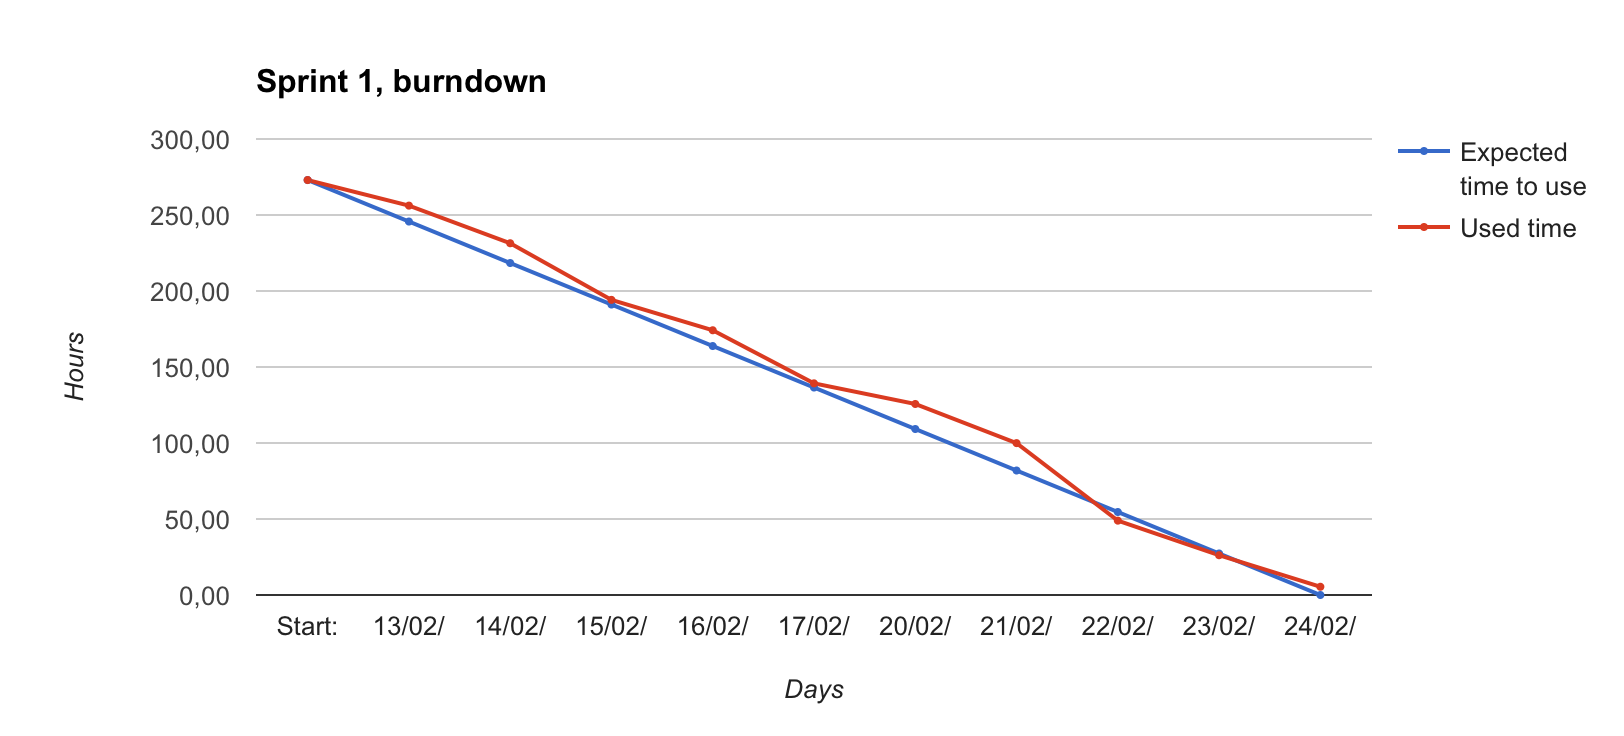
\includegraphics[width=0.8\textwidth]{fig/sprint1}
\caption{Sprint 1, burndown}
\end{figure}

Sprint backlog, burndowncharts, sprint review

\subsubsection{Webserver vs. Webhotel}
The platform for the web portal stood between Webhotel or VPS - virtual private server.  The group had several meetings with the customer regarding this decision. The customer primarily wanted to use web hotel as hosting service and platform. The group proposed to use VPS because it gave a lot of benefits and not constraints like using web hotel would give. 

The group presented to use VPS because it allows for developing the graphical user interface faster and easier by allowing usage of library and frameworks, that webhotels doesn't.  Thus time and resources would be more efficiently allocated. Security is also higher with the use of VPS because it doesn't use a shared resource. If the web portal was hosted through a web hotel, the security of the page and its information would only be protect as much as the less secure webpage that also uses the same shared resource. Hosting on VPS would provide more security for the users of the web portal, and since the product potentially holds sensitive information about the users, security is not to be taken for granted.  Experience also played a part in the decision. The group has more experience with the usage of VPS compared to web hotels. 

Regarding functionality and the project requirements, the platform could be either one, but the usage of VPS would give a much easier development and allow usage of the best suitable technology for the given task. 

The group presented the customer with the proposal to use VPS instead of webhotel, and was engaged in a consulting meeting with the customer, outside developer and the group. The group emphasized that the usage of VPS was just a suggestion, and that it was up to the customer to choose. The project could be done with both.  

\section{Sprint 2}
Sprint backlog, burndowncharts, sprint review

\section{Sprint 3}
Sprint backlog, burndowncharts, sprint review

\section{Sprint 4}
Sprint backlog, burndowncharts, sprint review

\section{Sprint 5}
Sprint backlog, burndowncharts, sprint review

\cleardoublepage